\documentclass[a4paper]{book}
\usepackage{makeidx}
\usepackage{natbib}
\usepackage{graphicx}
\usepackage{multicol}
\usepackage{float}
\usepackage{listings}
\usepackage{color}
\usepackage{ifthen}
\usepackage[table]{xcolor}
\usepackage{textcomp}
\usepackage{alltt}
\usepackage{ifpdf}
\ifpdf
\usepackage[pdftex,
            pagebackref=true,
            colorlinks=true,
            linkcolor=blue,
            unicode
           ]{hyperref}
\else
\usepackage[ps2pdf,
            pagebackref=true,
            colorlinks=true,
            linkcolor=blue,
            unicode
           ]{hyperref}
\usepackage{pspicture}
\fi
\usepackage[utf8]{inputenc}
\usepackage{mathptmx}
\usepackage[scaled=.90]{helvet}
\usepackage{courier}
\usepackage{sectsty}
\usepackage[titles]{tocloft}
\usepackage{doxygen}
\lstset{language=C++,inputencoding=utf8,basicstyle=\footnotesize,breaklines=true,breakatwhitespace=true,tabsize=8,numbers=left }
\makeindex
\setcounter{tocdepth}{3}
\renewcommand{\footrulewidth}{0.4pt}
\renewcommand{\familydefault}{\sfdefault}
\hfuzz=15pt
\setlength{\emergencystretch}{15pt}
\hbadness=750
\tolerance=750
\begin{document}
\hypersetup{pageanchor=false,citecolor=blue}
\begin{titlepage}
\vspace*{7cm}
\begin{center}
{\Large \-Laboratorio4\-\_\-\-C\-L\-A\-S\-E\-S }\\
\vspace*{1cm}
{\large \-Generated by Doxygen 1.7.6.1}\\
\vspace*{0.5cm}
{\small Sat Sep 13 2014 17:14:01}\\
\end{center}
\end{titlepage}
\clearemptydoublepage
\pagenumbering{roman}
\tableofcontents
\clearemptydoublepage
\pagenumbering{arabic}
\hypersetup{pageanchor=true,citecolor=blue}
\chapter{\-Class \-Index}
\section{Bioviewer Class Hierarchy}
This inheritance list is sorted roughly, but not completely, alphabetically:\begin{CompactList}
\item \_\-triangle\-V\item bvh\item bvh\-Part\item file\-Not\-Found\item \contentsline{section}{material}{\pageref{classmaterial}}{}
\item \contentsline{section}{matrix16f}{\pageref{classmatrix16f}}{}
\item \contentsline{section}{matrix9f}{\pageref{classmatrix9f}}{}
\item \contentsline{section}{movable}{\pageref{classmovable}}{}
\begin{CompactList}
\item body\item \contentsline{section}{camera}{\pageref{classcamera}}{}
\item \contentsline{section}{light}{\pageref{classlight}}{}
\item \contentsline{section}{objloader}{\pageref{classobjloader}}{}
\item \contentsline{section}{rigid}{\pageref{classrigid}}{}
\end{CompactList}
\item \contentsline{section}{point\-Mass}{\pageref{classpointMass}}{}
\item triangle\-Ind\item uv\item \contentsline{section}{vector3f}{\pageref{classvector3f}}{}
\end{CompactList}

\chapter{\-Class \-Index}
\section{Bioviewer Compound List}
Here are the classes, structs, unions and interfaces with brief descriptions:\begin{CompactList}
\item\contentsline{section}{{\bf camera} (Hold location and orientation of the viewer)}{\pageref{classcamera}}{}
\item\contentsline{section}{{\bf light} (Simple light point source)}{\pageref{classlight}}{}
\item\contentsline{section}{{\bf material} (Holds all vertices and material info for {\bf objloader} {\rm (p.\,\pageref{classobjloader})} entities)}{\pageref{classmaterial}}{}
\item\contentsline{section}{{\bf matrix16f} (Array of 16 floats in Open\-GL conformant style)}{\pageref{classmatrix16f}}{}
\item\contentsline{section}{{\bf matrix9f} (Smaller matrix for storing orientation but no location information)}{\pageref{classmatrix9f}}{}
\item\contentsline{section}{{\bf movable} (Mostly virtual class for any entity in the scene)}{\pageref{classmovable}}{}
\item\contentsline{section}{{\bf objloader} (Parse in .obj's)}{\pageref{classobjloader}}{}
\item\contentsline{section}{{\bf point\-Mass} (Generally attached to any number of springs)}{\pageref{classpointMass}}{}
\item\contentsline{section}{{\bf rigid} (Hold rigid body data, use {\bf objloader} {\rm (p.\,\pageref{classobjloader})} to load obj's)}{\pageref{classrigid}}{}
\item\contentsline{section}{{\bf vector3f} (Three floats in a array, lots of overloaded operators)}{\pageref{classvector3f}}{}
\end{CompactList}

\chapter{\-File \-Index}
\section{\-File \-List}
\-Here is a list of all files with brief descriptions\-:\begin{DoxyCompactList}
\item\contentsline{section}{\hyperlink{circulo_8cpp}{circulo.\-cpp} }{\pageref{circulo_8cpp}}{}
\item\contentsline{section}{\hyperlink{circulo_8hh}{circulo.\-hh} }{\pageref{circulo_8hh}}{}
\item\contentsline{section}{\hyperlink{cuadrado_8cpp}{cuadrado.\-cpp} }{\pageref{cuadrado_8cpp}}{}
\item\contentsline{section}{\hyperlink{cuadrado_8hh}{cuadrado.\-hh} }{\pageref{cuadrado_8hh}}{}
\item\contentsline{section}{\hyperlink{figura_8cpp}{figura.\-cpp} }{\pageref{figura_8cpp}}{}
\item\contentsline{section}{\hyperlink{figura_8hh}{figura.\-hh} }{\pageref{figura_8hh}}{}
\item\contentsline{section}{\hyperlink{principal_8cpp}{principal.\-cpp} }{\pageref{principal_8cpp}}{}
\item\contentsline{section}{\hyperlink{triangulo_8cpp}{triangulo.\-cpp} }{\pageref{triangulo_8cpp}}{}
\item\contentsline{section}{\hyperlink{triangulo_8hh}{triangulo.\-hh} }{\pageref{triangulo_8hh}}{}
\end{DoxyCompactList}

\chapter{\-Class \-Documentation}
\hypertarget{class_mi_circulo}{\section{\-Mi\-Circulo \-Class \-Reference}
\label{class_mi_circulo}\index{\-Mi\-Circulo@{\-Mi\-Circulo}}
}


{\ttfamily \#include $<$circulo.\-hh$>$}

\-Inheritance diagram for \-Mi\-Circulo\-:\begin{figure}[H]
\begin{center}
\leavevmode
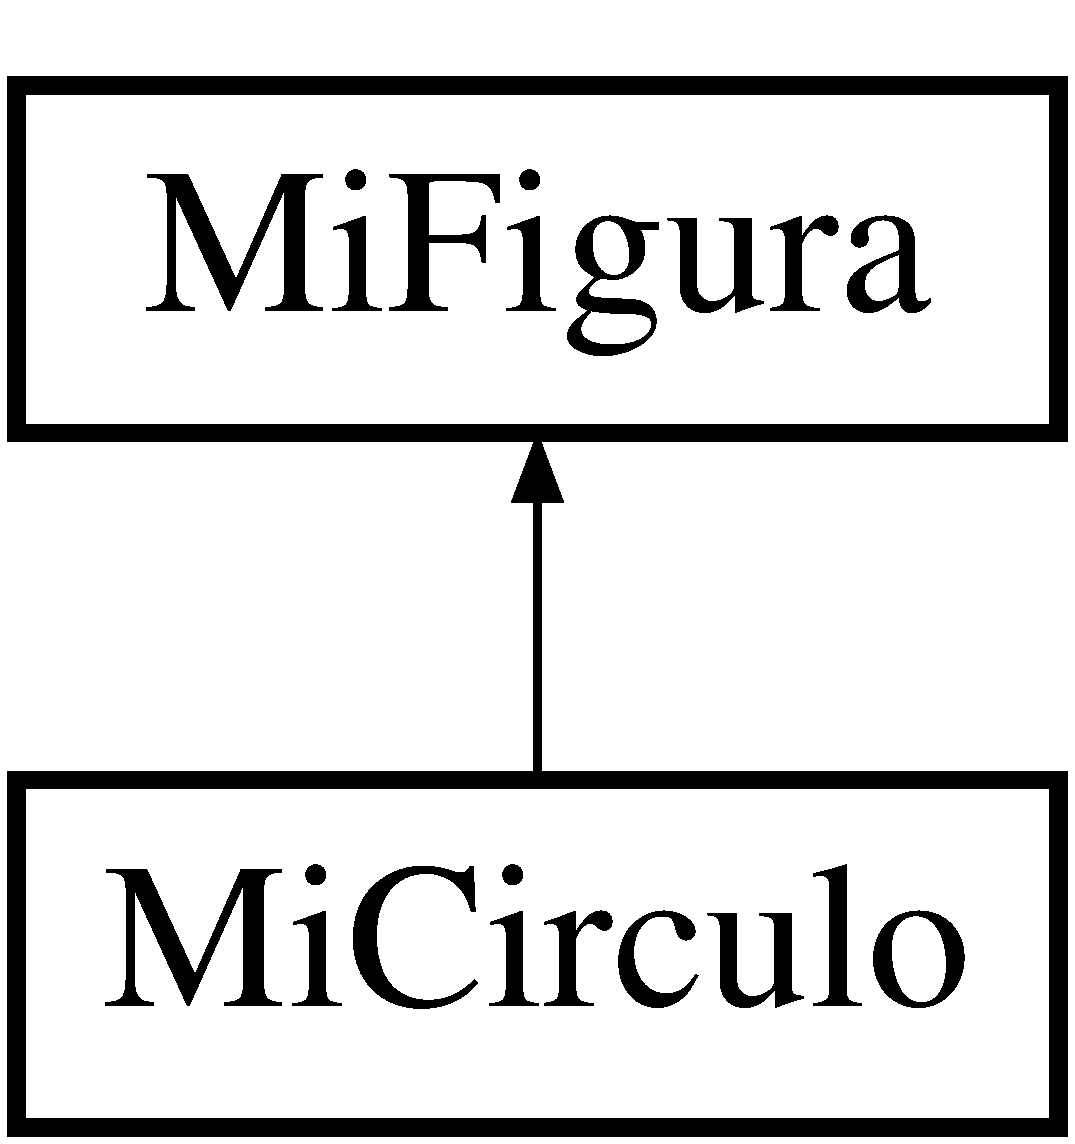
\includegraphics[height=2.000000cm]{class_mi_circulo}
\end{center}
\end{figure}
\subsection*{\-Public \-Member \-Functions}
\begin{DoxyCompactItemize}
\item 
\hyperlink{class_mi_circulo_a853aca73d0652d62ef59595eef7405da}{\-Mi\-Circulo} (void)
\begin{DoxyCompactList}\small\item\em \-Programa \hyperlink{circulo_8cpp}{circulo.\-cpp}. \end{DoxyCompactList}\item 
bool \hyperlink{class_mi_circulo_aace1e57cce1cb36ad353a3140af25d22}{area} (void)
\item 
bool \hyperlink{class_mi_circulo_affcbecc596851dc6ab3060dd9995eebd}{perimetro} (void)
\end{DoxyCompactItemize}


\subsection{\-Constructor \& \-Destructor \-Documentation}
\hypertarget{class_mi_circulo_a853aca73d0652d62ef59595eef7405da}{\index{\-Mi\-Circulo@{\-Mi\-Circulo}!\-Mi\-Circulo@{\-Mi\-Circulo}}
\index{\-Mi\-Circulo@{\-Mi\-Circulo}!MiCirculo@{\-Mi\-Circulo}}
\subsubsection[{\-Mi\-Circulo}]{\setlength{\rightskip}{0pt plus 5cm}{\bf \-Mi\-Circulo\-::\-Mi\-Circulo} (
\begin{DoxyParamCaption}
\item[{void}]{}
\end{DoxyParamCaption}
)}}\label{class_mi_circulo_a853aca73d0652d62ef59595eef7405da}


\-Programa \hyperlink{circulo_8cpp}{circulo.\-cpp}. 

\-Este programa se encarga de definir los métodos declarados en la libreria correspondiente \char`\"{}circulo.\-hh\char`\"{}. \-Constructor

\-Este es el constructor del programa y no recibe ningún parámetro.

\subsection{\-Member \-Function \-Documentation}
\hypertarget{class_mi_circulo_aace1e57cce1cb36ad353a3140af25d22}{\index{\-Mi\-Circulo@{\-Mi\-Circulo}!area@{area}}
\index{area@{area}!MiCirculo@{\-Mi\-Circulo}}
\subsubsection[{area}]{\setlength{\rightskip}{0pt plus 5cm}bool {\bf \-Mi\-Circulo\-::area} (
\begin{DoxyParamCaption}
\item[{void}]{}
\end{DoxyParamCaption}
)\hspace{0.3cm}{\ttfamily  \mbox{[}virtual\mbox{]}}}}\label{class_mi_circulo_aace1e57cce1cb36ad353a3140af25d22}
método area

\-Este método se encarga de mostrar en pantalla la fórmula para calcular el área de un circulo.

\-Reimplemented from \hyperlink{class_mi_figura_a337ca854a1149b8ed4dfbccae0b0c2d9}{\-Mi\-Figura}.

\hypertarget{class_mi_circulo_affcbecc596851dc6ab3060dd9995eebd}{\index{\-Mi\-Circulo@{\-Mi\-Circulo}!perimetro@{perimetro}}
\index{perimetro@{perimetro}!MiCirculo@{\-Mi\-Circulo}}
\subsubsection[{perimetro}]{\setlength{\rightskip}{0pt plus 5cm}bool {\bf \-Mi\-Circulo\-::perimetro} (
\begin{DoxyParamCaption}
\item[{void}]{}
\end{DoxyParamCaption}
)\hspace{0.3cm}{\ttfamily  \mbox{[}virtual\mbox{]}}}}\label{class_mi_circulo_affcbecc596851dc6ab3060dd9995eebd}
método perímetro

\-Este método se encarga de mostrar en pantalla la fórmula para calcular el perímetro de un circulo.

\-Reimplemented from \hyperlink{class_mi_figura_a8878d26a1623c513fbd8afa7181a72c9}{\-Mi\-Figura}.



\-The documentation for this class was generated from the following files\-:\begin{DoxyCompactItemize}
\item 
\hyperlink{circulo_8hh}{circulo.\-hh}\item 
\hyperlink{circulo_8cpp}{circulo.\-cpp}\end{DoxyCompactItemize}

\hypertarget{class_mi_cuadrado}{\section{\-Mi\-Cuadrado \-Class \-Reference}
\label{class_mi_cuadrado}\index{\-Mi\-Cuadrado@{\-Mi\-Cuadrado}}
}


{\ttfamily \#include $<$cuadrado.\-hh$>$}

\-Inheritance diagram for \-Mi\-Cuadrado\-:\begin{figure}[H]
\begin{center}
\leavevmode
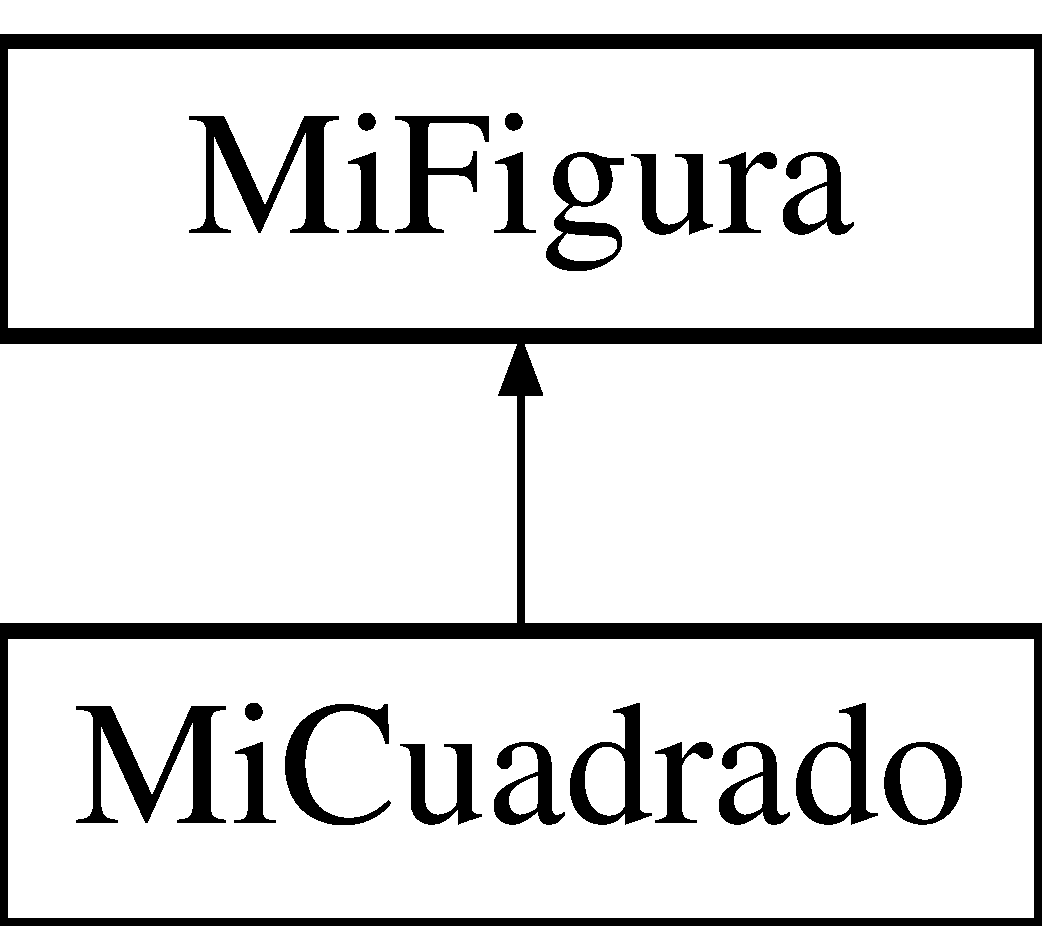
\includegraphics[height=2.000000cm]{class_mi_cuadrado}
\end{center}
\end{figure}
\subsection*{\-Public \-Member \-Functions}
\begin{DoxyCompactItemize}
\item 
\hyperlink{class_mi_cuadrado_a29faa030037d4a8511b9f36485c3c841}{\-Mi\-Cuadrado} (void)
\begin{DoxyCompactList}\small\item\em \-Programa \-Cuadrado.\-cpp. \end{DoxyCompactList}\item 
bool \hyperlink{class_mi_cuadrado_ae897b754e07d3d628ba6fbd339d4a477}{area} (void)
\item 
bool \hyperlink{class_mi_cuadrado_a1bfba7318b3cad1137b4900e0d156e76}{perimetro} (void)
\end{DoxyCompactItemize}


\subsection{\-Constructor \& \-Destructor \-Documentation}
\hypertarget{class_mi_cuadrado_a29faa030037d4a8511b9f36485c3c841}{\index{\-Mi\-Cuadrado@{\-Mi\-Cuadrado}!\-Mi\-Cuadrado@{\-Mi\-Cuadrado}}
\index{\-Mi\-Cuadrado@{\-Mi\-Cuadrado}!MiCuadrado@{\-Mi\-Cuadrado}}
\subsubsection[{\-Mi\-Cuadrado}]{\setlength{\rightskip}{0pt plus 5cm}{\bf \-Mi\-Cuadrado\-::\-Mi\-Cuadrado} (
\begin{DoxyParamCaption}
\item[{void}]{}
\end{DoxyParamCaption}
)}}\label{class_mi_cuadrado_a29faa030037d4a8511b9f36485c3c841}


\-Programa \-Cuadrado.\-cpp. 

\-Este programa se encarga de definir los métodos declarados en la libreria correspondiente \char`\"{}cuadrado.\-hh\char`\"{}. \-Constructor

\-Este es el constructor del programa y no recibe ningún parámetro.

\subsection{\-Member \-Function \-Documentation}
\hypertarget{class_mi_cuadrado_ae897b754e07d3d628ba6fbd339d4a477}{\index{\-Mi\-Cuadrado@{\-Mi\-Cuadrado}!area@{area}}
\index{area@{area}!MiCuadrado@{\-Mi\-Cuadrado}}
\subsubsection[{area}]{\setlength{\rightskip}{0pt plus 5cm}bool {\bf \-Mi\-Cuadrado\-::area} (
\begin{DoxyParamCaption}
\item[{void}]{}
\end{DoxyParamCaption}
)\hspace{0.3cm}{\ttfamily  \mbox{[}virtual\mbox{]}}}}\label{class_mi_cuadrado_ae897b754e07d3d628ba6fbd339d4a477}
método area

\-Este método se encarga de mostrar en pantalla la fórmula para calcular el área de un cuadrado.

\-Reimplemented from \hyperlink{class_mi_figura_a337ca854a1149b8ed4dfbccae0b0c2d9}{\-Mi\-Figura}.

\hypertarget{class_mi_cuadrado_a1bfba7318b3cad1137b4900e0d156e76}{\index{\-Mi\-Cuadrado@{\-Mi\-Cuadrado}!perimetro@{perimetro}}
\index{perimetro@{perimetro}!MiCuadrado@{\-Mi\-Cuadrado}}
\subsubsection[{perimetro}]{\setlength{\rightskip}{0pt plus 5cm}bool {\bf \-Mi\-Cuadrado\-::perimetro} (
\begin{DoxyParamCaption}
\item[{void}]{}
\end{DoxyParamCaption}
)\hspace{0.3cm}{\ttfamily  \mbox{[}virtual\mbox{]}}}}\label{class_mi_cuadrado_a1bfba7318b3cad1137b4900e0d156e76}
método perímetro

\-Este método se encarga de mostrar en pantalla la fórmula para calcular el perímetro de un cuadrado.

\-Reimplemented from \hyperlink{class_mi_figura_a8878d26a1623c513fbd8afa7181a72c9}{\-Mi\-Figura}.



\-The documentation for this class was generated from the following files\-:\begin{DoxyCompactItemize}
\item 
\hyperlink{cuadrado_8hh}{cuadrado.\-hh}\item 
\hyperlink{cuadrado_8cpp}{cuadrado.\-cpp}\end{DoxyCompactItemize}

\hypertarget{class_mi_figura}{\section{\-Mi\-Figura \-Class \-Reference}
\label{class_mi_figura}\index{\-Mi\-Figura@{\-Mi\-Figura}}
}


{\ttfamily \#include $<$figura.\-hh$>$}

\-Inheritance diagram for \-Mi\-Figura\-:\begin{figure}[H]
\begin{center}
\leavevmode
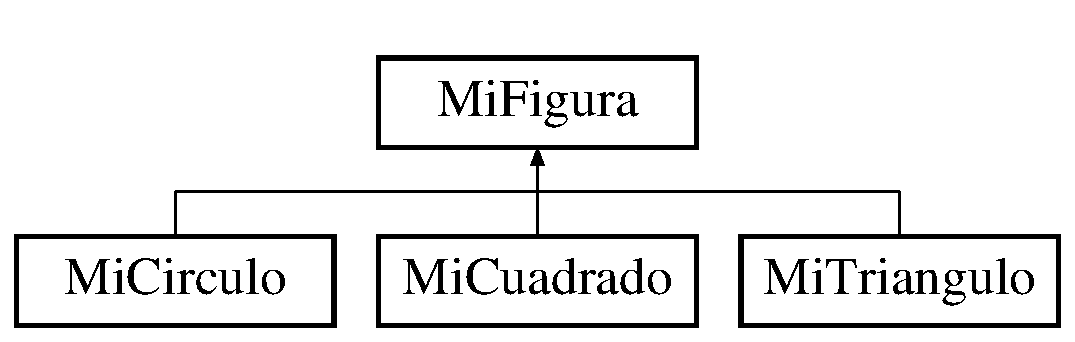
\includegraphics[height=2.000000cm]{class_mi_figura}
\end{center}
\end{figure}
\subsection*{\-Public \-Member \-Functions}
\begin{DoxyCompactItemize}
\item 
\hyperlink{class_mi_figura_ae56b70317f85507263e53b89878c0f9a}{\-Mi\-Figura} (string mi\-Nombre)
\begin{DoxyCompactList}\small\item\em \hyperlink{figura_8cpp}{figura.\-cpp} \end{DoxyCompactList}\item 
virtual \hyperlink{class_mi_figura_a84c77f42e83b2ef2489de98d31d2dd94}{$\sim$\-Mi\-Figura} (void)
\item 
bool \hyperlink{class_mi_figura_ae27e391b4a1a476d5d6f1f5c8be32f7e}{dibujar} (void)
\item 
virtual bool \hyperlink{class_mi_figura_a2592d5c4828ffcd3dfefe2b4180f1450}{mover} (void)
\item 
bool \hyperlink{class_mi_figura_a216858fd3c3da657743b9757d81c24f0}{borrar} (void)
\item 
virtual bool \hyperlink{class_mi_figura_a337ca854a1149b8ed4dfbccae0b0c2d9}{area} (void)
\item 
virtual bool \hyperlink{class_mi_figura_a8878d26a1623c513fbd8afa7181a72c9}{perimetro} (void)
\end{DoxyCompactItemize}
\subsection*{\-Protected \-Attributes}
\begin{DoxyCompactItemize}
\item 
string \hyperlink{class_mi_figura_a64efa122e4549b9c86c3053a6b5627df}{nombre}
\end{DoxyCompactItemize}


\subsection{\-Constructor \& \-Destructor \-Documentation}
\hypertarget{class_mi_figura_ae56b70317f85507263e53b89878c0f9a}{\index{\-Mi\-Figura@{\-Mi\-Figura}!\-Mi\-Figura@{\-Mi\-Figura}}
\index{\-Mi\-Figura@{\-Mi\-Figura}!MiFigura@{\-Mi\-Figura}}
\subsubsection[{\-Mi\-Figura}]{\setlength{\rightskip}{0pt plus 5cm}{\bf \-Mi\-Figura\-::\-Mi\-Figura} (
\begin{DoxyParamCaption}
\item[{string}]{mi\-Nombre}
\end{DoxyParamCaption}
)}}\label{class_mi_figura_ae56b70317f85507263e53b89878c0f9a}


\hyperlink{figura_8cpp}{figura.\-cpp} 

\-Este programa contiene la deficion de los métodos declarados en la clase figura. \-Constructor de \-Mifigura

\-Este constructor recibe como parametro un \char`\"{}string\char`\"{}, que cumple la función de nombre o identificador al nuevo nuevo objeto creado.\hypertarget{class_mi_figura_a84c77f42e83b2ef2489de98d31d2dd94}{\index{\-Mi\-Figura@{\-Mi\-Figura}!$\sim$\-Mi\-Figura@{$\sim$\-Mi\-Figura}}
\index{$\sim$\-Mi\-Figura@{$\sim$\-Mi\-Figura}!MiFigura@{\-Mi\-Figura}}
\subsubsection[{$\sim$\-Mi\-Figura}]{\setlength{\rightskip}{0pt plus 5cm}{\bf \-Mi\-Figura\-::$\sim$\-Mi\-Figura} (
\begin{DoxyParamCaption}
\item[{void}]{}
\end{DoxyParamCaption}
)\hspace{0.3cm}{\ttfamily  \mbox{[}virtual\mbox{]}}}}\label{class_mi_figura_a84c77f42e83b2ef2489de98d31d2dd94}
\-Desonstructor de \-Mifigura

\-Este desconstructor no recibe nungún parametro y simplemente desplega en la pantalla el aviso de que ha eliminado el objeto

\subsection{\-Member \-Function \-Documentation}
\hypertarget{class_mi_figura_a337ca854a1149b8ed4dfbccae0b0c2d9}{\index{\-Mi\-Figura@{\-Mi\-Figura}!area@{area}}
\index{area@{area}!MiFigura@{\-Mi\-Figura}}
\subsubsection[{area}]{\setlength{\rightskip}{0pt plus 5cm}virtual bool {\bf \-Mi\-Figura\-::area} (
\begin{DoxyParamCaption}
\item[{void}]{}
\end{DoxyParamCaption}
)\hspace{0.3cm}{\ttfamily  \mbox{[}inline, virtual\mbox{]}}}}\label{class_mi_figura_a337ca854a1149b8ed4dfbccae0b0c2d9}


\-Reimplemented in \hyperlink{class_mi_circulo_aace1e57cce1cb36ad353a3140af25d22}{\-Mi\-Circulo}, \hyperlink{class_mi_cuadrado_ae897b754e07d3d628ba6fbd339d4a477}{\-Mi\-Cuadrado}, and \hyperlink{class_mi_triangulo_a6c79d03804dfd5796c7c9de9bf4a2898}{\-Mi\-Triangulo}.

\hypertarget{class_mi_figura_a216858fd3c3da657743b9757d81c24f0}{\index{\-Mi\-Figura@{\-Mi\-Figura}!borrar@{borrar}}
\index{borrar@{borrar}!MiFigura@{\-Mi\-Figura}}
\subsubsection[{borrar}]{\setlength{\rightskip}{0pt plus 5cm}bool {\bf \-Mi\-Figura\-::borrar} (
\begin{DoxyParamCaption}
\item[{void}]{}
\end{DoxyParamCaption}
)}}\label{class_mi_figura_a216858fd3c3da657743b9757d81c24f0}
método borrar

\-Este método se encarga de mostrar en pantalla la palabra \char`\"{}borrando\char`\"{}\hypertarget{class_mi_figura_ae27e391b4a1a476d5d6f1f5c8be32f7e}{\index{\-Mi\-Figura@{\-Mi\-Figura}!dibujar@{dibujar}}
\index{dibujar@{dibujar}!MiFigura@{\-Mi\-Figura}}
\subsubsection[{dibujar}]{\setlength{\rightskip}{0pt plus 5cm}bool {\bf \-Mi\-Figura\-::dibujar} (
\begin{DoxyParamCaption}
\item[{void}]{}
\end{DoxyParamCaption}
)}}\label{class_mi_figura_ae27e391b4a1a476d5d6f1f5c8be32f7e}
método dibujar

\-Este método se encarga de mostrar en pantalla la palabra \char`\"{}dibujando\char`\"{}\hypertarget{class_mi_figura_a2592d5c4828ffcd3dfefe2b4180f1450}{\index{\-Mi\-Figura@{\-Mi\-Figura}!mover@{mover}}
\index{mover@{mover}!MiFigura@{\-Mi\-Figura}}
\subsubsection[{mover}]{\setlength{\rightskip}{0pt plus 5cm}bool {\bf \-Mi\-Figura\-::mover} (
\begin{DoxyParamCaption}
\item[{void}]{}
\end{DoxyParamCaption}
)\hspace{0.3cm}{\ttfamily  \mbox{[}virtual\mbox{]}}}}\label{class_mi_figura_a2592d5c4828ffcd3dfefe2b4180f1450}
método mover

\-Este método se encarga de mostrar en pantalla la palabra \char`\"{}moviendo\char`\"{}\hypertarget{class_mi_figura_a8878d26a1623c513fbd8afa7181a72c9}{\index{\-Mi\-Figura@{\-Mi\-Figura}!perimetro@{perimetro}}
\index{perimetro@{perimetro}!MiFigura@{\-Mi\-Figura}}
\subsubsection[{perimetro}]{\setlength{\rightskip}{0pt plus 5cm}virtual bool {\bf \-Mi\-Figura\-::perimetro} (
\begin{DoxyParamCaption}
\item[{void}]{}
\end{DoxyParamCaption}
)\hspace{0.3cm}{\ttfamily  \mbox{[}inline, virtual\mbox{]}}}}\label{class_mi_figura_a8878d26a1623c513fbd8afa7181a72c9}


\-Reimplemented in \hyperlink{class_mi_circulo_affcbecc596851dc6ab3060dd9995eebd}{\-Mi\-Circulo}, \hyperlink{class_mi_cuadrado_a1bfba7318b3cad1137b4900e0d156e76}{\-Mi\-Cuadrado}, and \hyperlink{class_mi_triangulo_a1924fcfe9d32b1b6b217cbb1d9ea7821}{\-Mi\-Triangulo}.



\subsection{\-Member \-Data \-Documentation}
\hypertarget{class_mi_figura_a64efa122e4549b9c86c3053a6b5627df}{\index{\-Mi\-Figura@{\-Mi\-Figura}!nombre@{nombre}}
\index{nombre@{nombre}!MiFigura@{\-Mi\-Figura}}
\subsubsection[{nombre}]{\setlength{\rightskip}{0pt plus 5cm}string {\bf \-Mi\-Figura\-::nombre}\hspace{0.3cm}{\ttfamily  \mbox{[}protected\mbox{]}}}}\label{class_mi_figura_a64efa122e4549b9c86c3053a6b5627df}


\-The documentation for this class was generated from the following files\-:\begin{DoxyCompactItemize}
\item 
\hyperlink{figura_8hh}{figura.\-hh}\item 
\hyperlink{figura_8cpp}{figura.\-cpp}\end{DoxyCompactItemize}

\hypertarget{class_mi_triangulo}{\section{\-Mi\-Triangulo \-Class \-Reference}
\label{class_mi_triangulo}\index{\-Mi\-Triangulo@{\-Mi\-Triangulo}}
}


{\ttfamily \#include $<$triangulo.\-hh$>$}

\-Inheritance diagram for \-Mi\-Triangulo\-:\begin{figure}[H]
\begin{center}
\leavevmode
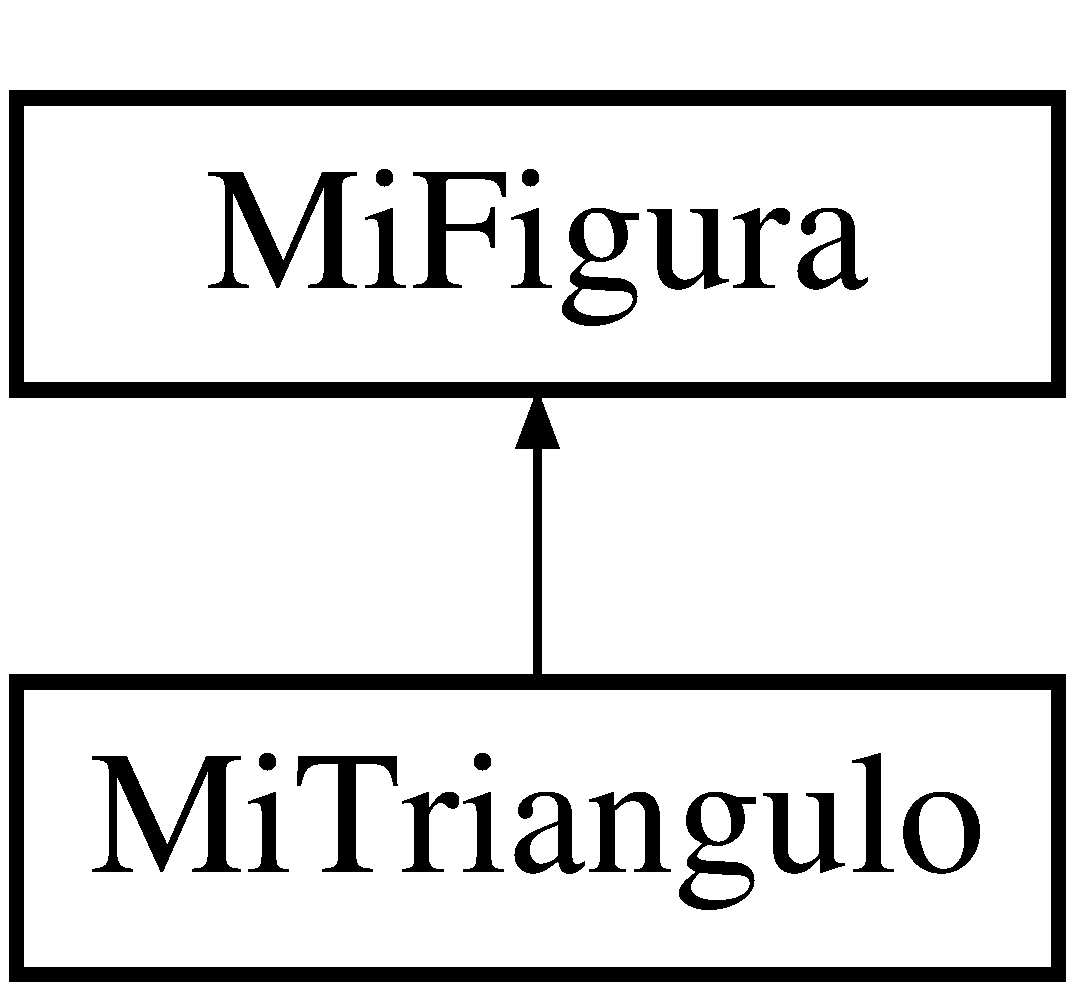
\includegraphics[height=2.000000cm]{class_mi_triangulo}
\end{center}
\end{figure}
\subsection*{\-Public \-Member \-Functions}
\begin{DoxyCompactItemize}
\item 
\hyperlink{class_mi_triangulo_ab9e93a152881b2ff30f2a03ed8c5acd8}{\-Mi\-Triangulo} (void)
\begin{DoxyCompactList}\small\item\em \-Programa \hyperlink{triangulo_8cpp}{triangulo.\-cpp}. \end{DoxyCompactList}\item 
bool \hyperlink{class_mi_triangulo_a6c79d03804dfd5796c7c9de9bf4a2898}{area} (void)
\item 
bool \hyperlink{class_mi_triangulo_a1924fcfe9d32b1b6b217cbb1d9ea7821}{perimetro} (void)
\item 
bool \hyperlink{class_mi_triangulo_a695fbaa82773786965aef90831939032}{girar\-Horizontal} (void)
\item 
bool \hyperlink{class_mi_triangulo_a15ee9f3600760ec7f7d4b83923965619}{girar\-Vertical} (void)
\end{DoxyCompactItemize}


\subsection{\-Constructor \& \-Destructor \-Documentation}
\hypertarget{class_mi_triangulo_ab9e93a152881b2ff30f2a03ed8c5acd8}{\index{\-Mi\-Triangulo@{\-Mi\-Triangulo}!\-Mi\-Triangulo@{\-Mi\-Triangulo}}
\index{\-Mi\-Triangulo@{\-Mi\-Triangulo}!MiTriangulo@{\-Mi\-Triangulo}}
\subsubsection[{\-Mi\-Triangulo}]{\setlength{\rightskip}{0pt plus 5cm}{\bf \-Mi\-Triangulo\-::\-Mi\-Triangulo} (
\begin{DoxyParamCaption}
\item[{void}]{}
\end{DoxyParamCaption}
)}}\label{class_mi_triangulo_ab9e93a152881b2ff30f2a03ed8c5acd8}


\-Programa \hyperlink{triangulo_8cpp}{triangulo.\-cpp}. 

\-Este programa se encarga de definir los métodos que se declararon en la libreria correspondiente \char`\"{}triangulo.\-hh\char`\"{} \-Contructos de \char`\"{}\-Mi\-Triangulo\char`\"{}

\-Este es el contructor del programa y no recibe ningún parámetro.

\subsection{\-Member \-Function \-Documentation}
\hypertarget{class_mi_triangulo_a6c79d03804dfd5796c7c9de9bf4a2898}{\index{\-Mi\-Triangulo@{\-Mi\-Triangulo}!area@{area}}
\index{area@{area}!MiTriangulo@{\-Mi\-Triangulo}}
\subsubsection[{area}]{\setlength{\rightskip}{0pt plus 5cm}bool {\bf \-Mi\-Triangulo\-::area} (
\begin{DoxyParamCaption}
\item[{void}]{}
\end{DoxyParamCaption}
)\hspace{0.3cm}{\ttfamily  \mbox{[}virtual\mbox{]}}}}\label{class_mi_triangulo_a6c79d03804dfd5796c7c9de9bf4a2898}
método area

\-Este método se encarga de mostrar en pantalla la fórmula para para calcular el area de un triangulo.

\-Reimplemented from \hyperlink{class_mi_figura_a337ca854a1149b8ed4dfbccae0b0c2d9}{\-Mi\-Figura}.

\hypertarget{class_mi_triangulo_a695fbaa82773786965aef90831939032}{\index{\-Mi\-Triangulo@{\-Mi\-Triangulo}!girar\-Horizontal@{girar\-Horizontal}}
\index{girar\-Horizontal@{girar\-Horizontal}!MiTriangulo@{\-Mi\-Triangulo}}
\subsubsection[{girar\-Horizontal}]{\setlength{\rightskip}{0pt plus 5cm}bool {\bf \-Mi\-Triangulo\-::girar\-Horizontal} (
\begin{DoxyParamCaption}
\item[{void}]{}
\end{DoxyParamCaption}
)}}\label{class_mi_triangulo_a695fbaa82773786965aef90831939032}
método girar\-Horizontal

\-Este método se encarga de mostrar en pantalla la frase \char`\"{}se giró horizontalmente\char`\"{}.\hypertarget{class_mi_triangulo_a15ee9f3600760ec7f7d4b83923965619}{\index{\-Mi\-Triangulo@{\-Mi\-Triangulo}!girar\-Vertical@{girar\-Vertical}}
\index{girar\-Vertical@{girar\-Vertical}!MiTriangulo@{\-Mi\-Triangulo}}
\subsubsection[{girar\-Vertical}]{\setlength{\rightskip}{0pt plus 5cm}bool {\bf \-Mi\-Triangulo\-::girar\-Vertical} (
\begin{DoxyParamCaption}
\item[{void}]{}
\end{DoxyParamCaption}
)}}\label{class_mi_triangulo_a15ee9f3600760ec7f7d4b83923965619}
método girar\-Vertical

\-Este método se encarga de mostrar en pantalla la frase \char`\"{}se giró verticalmente\char`\"{}.\hypertarget{class_mi_triangulo_a1924fcfe9d32b1b6b217cbb1d9ea7821}{\index{\-Mi\-Triangulo@{\-Mi\-Triangulo}!perimetro@{perimetro}}
\index{perimetro@{perimetro}!MiTriangulo@{\-Mi\-Triangulo}}
\subsubsection[{perimetro}]{\setlength{\rightskip}{0pt plus 5cm}bool {\bf \-Mi\-Triangulo\-::perimetro} (
\begin{DoxyParamCaption}
\item[{void}]{}
\end{DoxyParamCaption}
)\hspace{0.3cm}{\ttfamily  \mbox{[}virtual\mbox{]}}}}\label{class_mi_triangulo_a1924fcfe9d32b1b6b217cbb1d9ea7821}
método perímetro

\-Este método se encarga de mostrar en pantalla la fórmula para para calcular el perímetro de un triangulo.

\-Reimplemented from \hyperlink{class_mi_figura_a8878d26a1623c513fbd8afa7181a72c9}{\-Mi\-Figura}.



\-The documentation for this class was generated from the following files\-:\begin{DoxyCompactItemize}
\item 
\hyperlink{triangulo_8hh}{triangulo.\-hh}\item 
\hyperlink{triangulo_8cpp}{triangulo.\-cpp}\end{DoxyCompactItemize}

\chapter{\-File \-Documentation}
\hypertarget{circulo_8cpp}{\section{circulo.\-cpp \-File \-Reference}
\label{circulo_8cpp}\index{circulo.\-cpp@{circulo.\-cpp}}
}
{\ttfamily \#include \char`\"{}circulo.\-hh\char`\"{}}\*

\hypertarget{circulo_8hh}{\section{circulo.\-hh \-File \-Reference}
\label{circulo_8hh}\index{circulo.\-hh@{circulo.\-hh}}
}
{\ttfamily \#include \char`\"{}figura.\-hh\char`\"{}}\*
\subsection*{\-Classes}
\begin{DoxyCompactItemize}
\item 
class \hyperlink{class_mi_circulo}{\-Mi\-Circulo}
\end{DoxyCompactItemize}

\hypertarget{cuadrado_8cpp}{\section{cuadrado.\-cpp \-File \-Reference}
\label{cuadrado_8cpp}\index{cuadrado.\-cpp@{cuadrado.\-cpp}}
}
{\ttfamily \#include \char`\"{}cuadrado.\-hh\char`\"{}}\*

\hypertarget{cuadrado_8hh}{\section{cuadrado.\-hh \-File \-Reference}
\label{cuadrado_8hh}\index{cuadrado.\-hh@{cuadrado.\-hh}}
}
{\ttfamily \#include \char`\"{}figura.\-hh\char`\"{}}\*
\subsection*{\-Classes}
\begin{DoxyCompactItemize}
\item 
class \hyperlink{class_mi_cuadrado}{\-Mi\-Cuadrado}
\end{DoxyCompactItemize}

\hypertarget{figura_8cpp}{\section{figura.\-cpp \-File \-Reference}
\label{figura_8cpp}\index{figura.\-cpp@{figura.\-cpp}}
}
{\ttfamily \#include \char`\"{}figura.\-hh\char`\"{}}\*

\hypertarget{figura_8hh}{\section{figura.\-hh \-File \-Reference}
\label{figura_8hh}\index{figura.\-hh@{figura.\-hh}}
}
{\ttfamily \#include $<$string$>$}\*
{\ttfamily \#include $<$iostream$>$}\*
\subsection*{\-Classes}
\begin{DoxyCompactItemize}
\item 
class \hyperlink{class_mi_figura}{\-Mi\-Figura}
\end{DoxyCompactItemize}

\hypertarget{principal_8cpp}{\section{principal.\-cpp \-File \-Reference}
\label{principal_8cpp}\index{principal.\-cpp@{principal.\-cpp}}
}
{\ttfamily \#include \char`\"{}circulo.\-hh\char`\"{}}\*
{\ttfamily \#include \char`\"{}triangulo.\-hh\char`\"{}}\*
{\ttfamily \#include \char`\"{}cuadrado.\-hh\char`\"{}}\*
\subsection*{\-Functions}
\begin{DoxyCompactItemize}
\item 
int \hyperlink{principal_8cpp_ae66f6b31b5ad750f1fe042a706a4e3d4}{main} ()
\end{DoxyCompactItemize}


\subsection{\-Function \-Documentation}
\hypertarget{principal_8cpp_ae66f6b31b5ad750f1fe042a706a4e3d4}{\index{principal.\-cpp@{principal.\-cpp}!main@{main}}
\index{main@{main}!principal.cpp@{principal.\-cpp}}
\subsubsection[{main}]{\setlength{\rightskip}{0pt plus 5cm}int {\bf main} (
\begin{DoxyParamCaption}
{}
\end{DoxyParamCaption}
)}}\label{principal_8cpp_ae66f6b31b5ad750f1fe042a706a4e3d4}

\hypertarget{triangulo_8cpp}{\section{triangulo.\-cpp \-File \-Reference}
\label{triangulo_8cpp}\index{triangulo.\-cpp@{triangulo.\-cpp}}
}
{\ttfamily \#include \char`\"{}triangulo.\-hh\char`\"{}}\*

\hypertarget{triangulo_8hh}{\section{triangulo.\-hh \-File \-Reference}
\label{triangulo_8hh}\index{triangulo.\-hh@{triangulo.\-hh}}
}
{\ttfamily \#include \char`\"{}figura.\-hh\char`\"{}}\*
\subsection*{\-Classes}
\begin{DoxyCompactItemize}
\item 
class \hyperlink{class_mi_triangulo}{\-Mi\-Triangulo}
\end{DoxyCompactItemize}

\printindex
\end{document}
